\documentclass[11pt, a4paper]{article}

\usepackage{graphicx}
\usepackage[a4paper,top=3cm,bottom=2cm,left=2cm,right=2cm,marginparwidth=1.75cm]{geometry}
\usepackage[english]{babel}
\usepackage[utf8x]{inputenc}
\usepackage{subfig}
\usepackage{float}
\usepackage{amsmath}
\usepackage{amssymb}
\usepackage{mhchem}
\usepackage{hyperref}
\usepackage{tikz}
\usepackage{cancel}
\usepackage{bm}

\graphicspath{ {./images} }
\newcommand*{\qed}{\hfill\ensuremath{\quad\square}}%
\newcommand*{\rad}{\ensuremath{\,\text{rad}}}
\newcommand*{\R}{\ensuremath{\mathbb{R}}}
\newcommand*{\C}{\ensuremath{\mathbb{C}}}
\renewcommand*{\Re}{\operatorname{Re}}
\renewcommand*{\Im}{\operatorname{Im}}
\renewcommand*{\epsilon}{\varepsilon}
\renewcommand*{\phi}{\varphi}
\renewcommand*{\d}{\text{d}}

\DeclareRobustCommand{\uvec}[1]{{%
  \ifcat\relax\noexpand#1%
    % it should be a Greek letter
    \bm{\hat{#1}}%
  \else
    \ifcsname uvec#1\endcsname
      \csname uvec#1\endcsname
    \else
      \bm{\hat{\mathbf{#1}}}%
     \fi
   \fi
}}

\makeatletter
\renewcommand*\env@matrix[1][*\c@MaxMatrixCols c]{%
  \hskip -\arraycolsep
  \let\@ifnextchar\new@ifnextchar
  \array{#1}}
\makeatother

\newtheorem{theorem}{Theorem}
\numberwithin{equation}{section}

%------------------------------------------------
%Templates for images and figures
% \begin{figure}[h]
%   \centering
%   \subfloat[caption 1]{{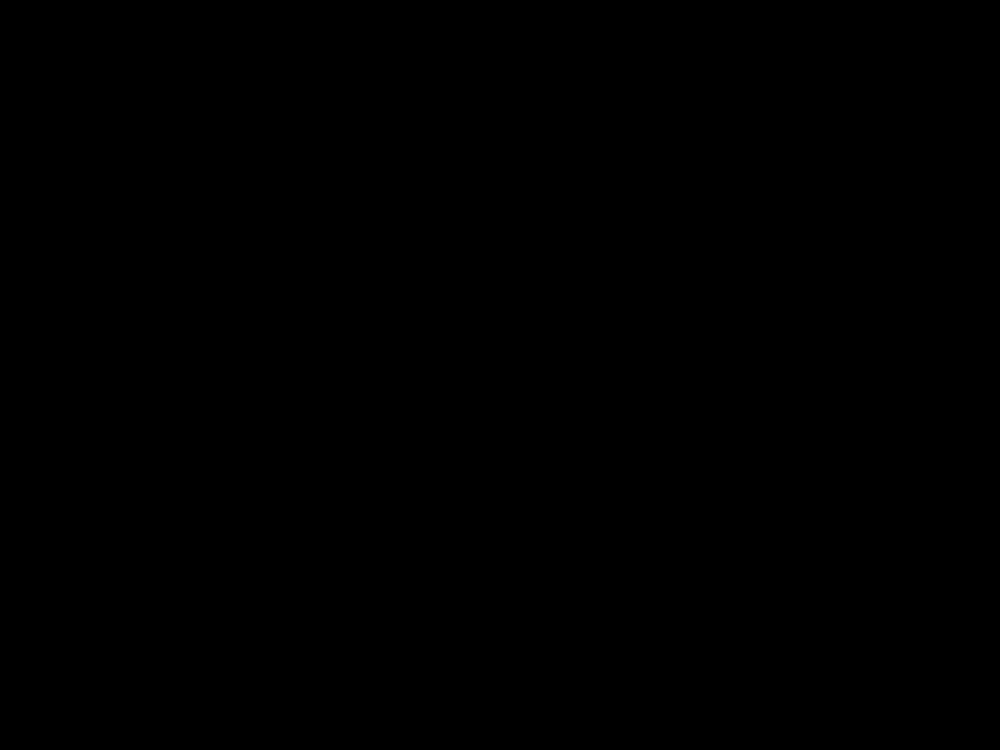
\includegraphics[width=30mm]{images/placeholder.png}}}%
%   \qquad
%   \subfloat[caption 2]{{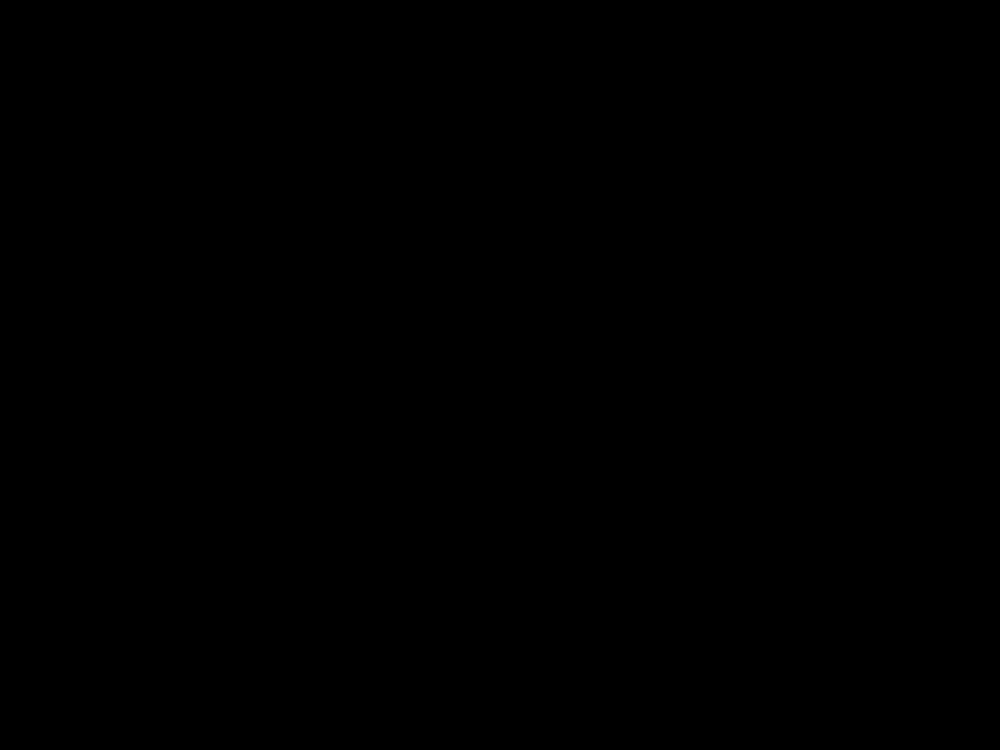
\includegraphics[width=30mm]{images/placeholder.png}}}%
%   \caption{Description}
% \end{figure}

% \begin{figure}[h]
%   \centerline{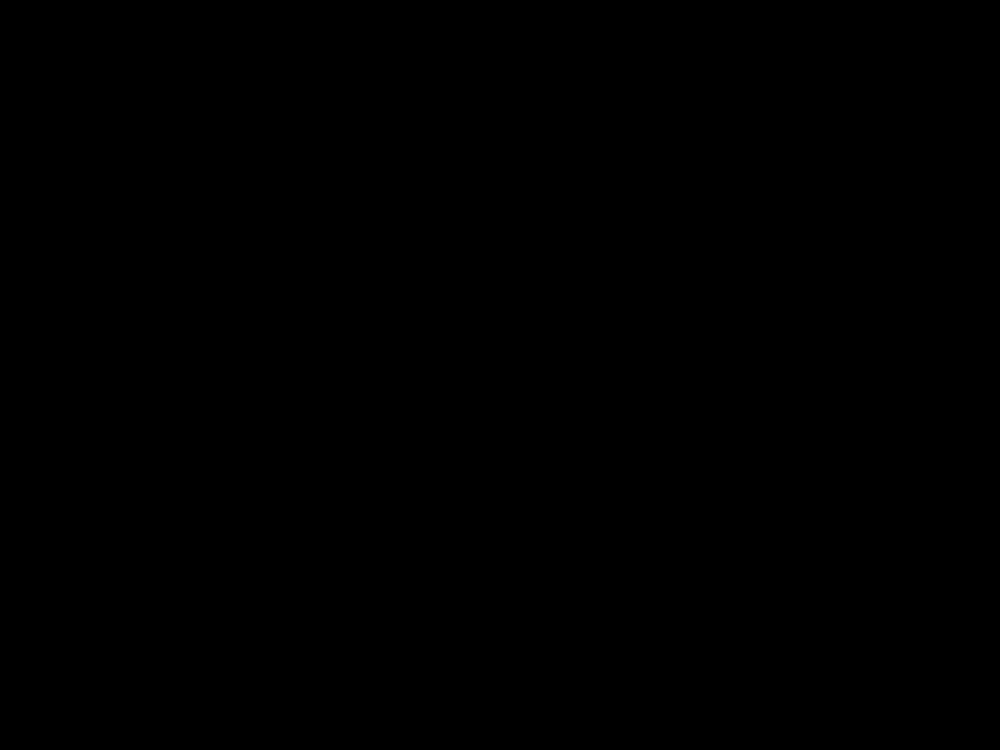
\includegraphics[width=50mm]{images/placeholder.png}}
%   \caption{Description}
% \end{figure}

%Template for a simple table 
%\begin{table}[h]
%   \caption{Description} %title of the table
%   \centering % centering table
%   \begin{tabular}{l rr} % creating three columns
%     \hline\hline %inserting double-line
%     & & \\ [0.5ex] % Insert half line vertical spacing
%     \hline % inserts single-line
%     & & \\ 
%     & & \\
%     & & \\
%     & & \\
%   \hline % inserts single-line
%   \end{tabular}
%   \label{tab:hresult}
% \end{table}
%-----------------------------------------------

\begin{document}
\section{Introduction to continuum mechanics}


\subsection{The continuum theory}
Steel when observed from afar looks like one homogeneous medium, however if we zoom in we find that the material, which initally looked smooth, has a crystalline structure. Zooming in a bit further then that we find that dislocations occur in the crystalline structure. Zooming in even further we find that the material is made up of individual atoms arranged in a lattice. When analysing a material we usually want to ignore details like crysltalline structure as this would make models very computationally expensive and too complex. So instead for the analysis we choose a volume element of the material which is sufficiently large, such that we interpret variables of interest as some mean value over a small discrete volume element. Describing materials this way is referred to as a \textbf{continuum description}.\\
Because of the continuum description variables such as strain, stress, temperature, displacement, etc. can be described as a continuous differentiable function. The continuous function represent the mean values of these variables for a small volume of material. This description is only valid if the fluctuation of these variables takes place at a scale which is large as compared to the material length scale.


\subsection{The basic equations in statics}
In statics we generally consider three distinct sets of equations:
\begin{enumerate}
  \item The requirements for continuity, a set of equations ensuring all material stays connected to itself without any discontinuities arising.
  \item Equilibrium, a set of equations which relates stress distributions and externally applied loads.
  \item Relating deformation and stress.
\end{enumerate}
This is often called a constitutive model. In general the computationally easiest way to go about this is the following order:\\
\begin{center}
  Displacements $\Rightarrow$ Deformations $\Rightarrow$ Stresses $\Rightarrow$ Extrernal Loads
\end{center}
The problem is: in statics we usually start with external loads, and we want to figure out what displacement these loads are causing.


\subsection{Continuity}
Consider a 3 dimensional body in undeformed and in deformed configuration as show in figure 1.1.
\begin{figure}[h]
  \centerline{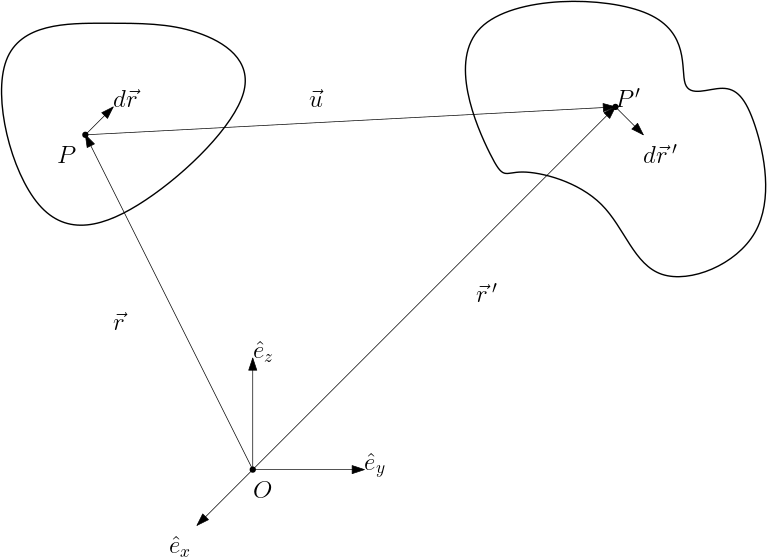
\includegraphics[width=100mm]{images/Deformation_example.png}}
  \caption{Representation of some patato shaped continuum in udeformed and in deformed configuration}
\end{figure}
The position vector from the origin to the material point $P$ can be given as:
\begin{equation}
  \vec{r} = x\uvec{e}_x + y\uvec{e}_y + z\uvec{e}_z
\end{equation}
When deformed the point $P$ will be transformed to the point $P'$. The vector from the origin to this new point $P'$ will be $\vec{r}\,'$. The vector $\vec{u}$ which is the position vector to point $P'$ with respect to point $P$ can then be given as follows:
\begin{equation}
  \vec{u} =  u_x\uvec{e}_x + u_y\uvec{e}_y + u_z\uvec{e}_z = \vec{r}\,' - \vec{r}
\end{equation}
Note that both the vectors $\vec{r}$ and $\vec{u}$ are vector valued functions of spatial coordinates:
\begin{align}
  \vec{u} &= \vec{u}(x, y, z)\\
  \vec{r} &= \vec{r}(x, y, z)
\end{align}
Now consider a differential element of the vector $\vec{r}$:
\begin{equation}
  \d\vec{r} = \d x\uvec{e}_x + \d y\uvec{e}_y + \d z\uvec{e}_z
\end{equation}
This vector represents a material element which is infinitesimally  close to the original point $P$. We consider the same point infinitesimally close to $P'$ with the unit vector $\vec{r}\,'$:
\begin{equation}
  \d \vec{r}\,' = \d(\vec{r} + \vec{u}) = \d\vec{r} + \d\vec{u}
\end{equation}
We can take a differential element of the vector $\vec{u}$ as:
\begin{equation}
  \d \vec{u} =  \d u_x\uvec{e}_x + \d u_y\uvec{e}_y + \d u_z\uvec{e}_z
\end{equation}
Where the terms $\d u_x$, $\d u_y$ and $\d u_z$ represent the deformation in the $x, y$ and $z$ direction. If we let this deformation 'act' on some position vector $\vec{r}$ to some point on the continuum we get:
\begin{align}
  \d u_x &= u_x(\vec{r}+\d \vec{r}) - u_x(\vec{r})\\
         &= \cancel{u_x} + \frac{\partial u_x}{\partial x}\d x + \frac{\partial u_x}{\partial y} 
            \d y + \frac{\partial u_x}{\partial z}\d z - \cancel{u_x}\\
         &= \frac{\partial u_x}{\partial x}\d x + \frac{\partial u_x}{\partial y} 
         \d y + \frac{\partial u_x}{\partial z}\d z
\end{align}

\end{document}